\documentclass[12pt,a4paper]{report}
\usepackage[utf8]{inputenc}
\usepackage[spanish]{babel}
\usepackage{amsmath}
\usepackage{amsfonts}
\usepackage{amssymb}
\usepackage{graphicx}
\usepackage{vmargin}

\usepackage[T1]{fontenc}  
\usepackage{titlesec}

\usepackage{hyperref}
\hypersetup{
    colorlinks=true,
    linkcolor=blue,
    filecolor=magenta,      
    urlcolor=blue,
}
 
\urlstyle{same}





\makeatletter
\author{Nombre de los integrantes :\\\\Eyssautier Hernández Michel Karina\\
Francisco Villaseñor Andrade\\
Pérez Hernández Magaly\\
Ponce García Alejandro\\
Reyes Bermúdez Natalia\\
Velasco Bazán Cecilio Omar\\
Ramírez Hernández Jonathan\\
Bárcenas Martínez Erick Iván
\\\\Profesor: M.I. José Luis Rodríguez Picazo}
\date{Ciudad de México, 21 de noviembre de 2019}
\title{Universidad Nacional Autónoma de México\\Facultad de Ingeniería\\Mecánica de Sólidos\\Proyecto final: Polipasto con trole fija al centro de travesaño}


\begin{document}
\maketitle


\chapter*{I. OBJETIVO}
Entregar el reporte con la evaluación de resultados para la realización de un proyecto teórico práctico durante el diseño de un elemento estructural propuesto, con la finalidad de comparar las salidas obtenidas en el modelo experimental contra las salidas esperadas del cálculo teórico, en términos de determinación e interpretación de esfuerzos y deformaciones.

\chapter*{II .ELEMENTO DE ANÁLISIS}
Modelo experimental a escala de un "Polipasto con trole fija al centro de \\travesaño", con longitud de tirante mínimo de 50 cm. y con capacidad para carga \\de 2.0 kg min. Altura libre.

\chapter*{III. SALIDAS TEÓRICAS Y EXPERIMENTALES}

\chapter{DISEÑO CONCEPTUAL ESTRUCTURAL}







\section{Cumplimiento de la especificación \\proporcionada.} % section headings are printed smaller than chapter names

\begin{figure}[h]
  \centering
    \includegraphics[width=\textwidth]{A/figs/A_1.jpg}  
    \caption{Superior} % should be 1.1
\end{figure}

\begin{figure}[h]
  \centering
    \includegraphics[width=\textwidth]{A/figs/A_2.jpg}  
    \caption{Inferior} % should be 2.1 - actually is 2 or 2.2 with optional code
\end{figure}
\ \ \ 
\section{Planos descriptivos de fabricación y ensamble.}



\begin{center}
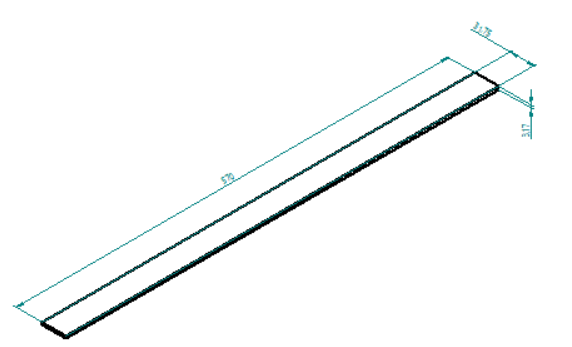
\includegraphics[width=.6\linewidth]{A/figs/B_1.png} 
 \includegraphics[width=.6\linewidth]{A/figs/B_2.png} 

\end{center}

\begin{center}
\includegraphics[width=1\linewidth]{A/figs/C_1.png} 
\end{center}

\begin{center}
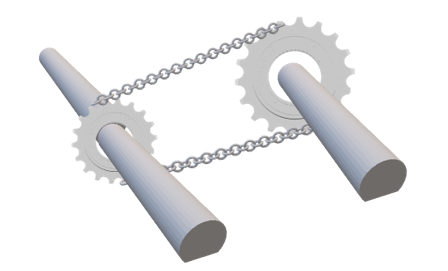
\includegraphics[width=.6\linewidth]{A/figs/C_2.png} 
\end{center}

\begin{center}
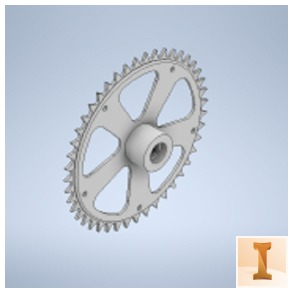
\includegraphics[width=.6\linewidth]{A/figs/elements/A_5.jpeg} 
 

\end{center}

\begin{center}
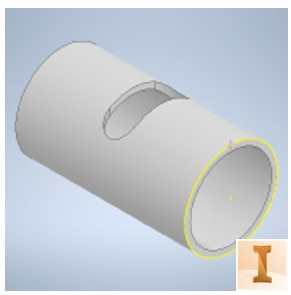
\includegraphics[width=.3\linewidth]{A/figs/elements/A_1.jpeg}  
\includegraphics[width=.3\linewidth]{A/figs/elements/A_2.jpeg}  
\includegraphics[width=.3\linewidth]{A/figs/elements/A_3.jpeg}
\\[\baselineskip]% adds vertical line spacing
\quad\includegraphics[width=.3\linewidth]{A/figs/elements/A_4.jpeg}  
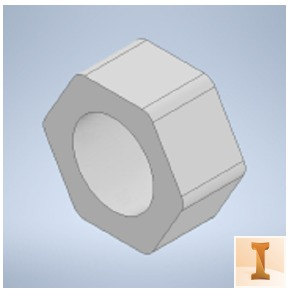
\includegraphics[width=.3\linewidth]{A/figs/elements/A_7.jpeg} 
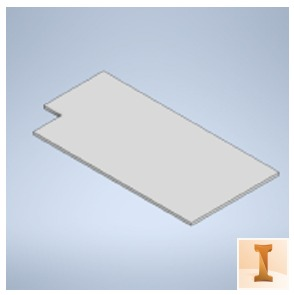
\includegraphics[width=.3\linewidth]{A/figs/elements/A_6.jpeg} 

\end{center}



\begin{center}
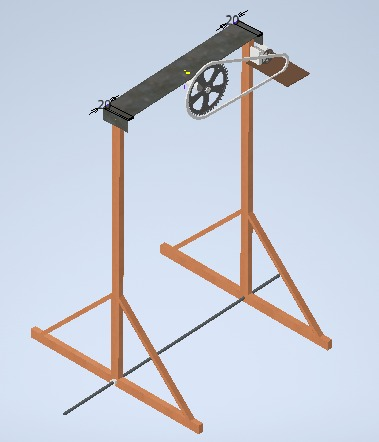
\includegraphics[width=.6\linewidth]{A/figs/elements/A_8.jpeg}  
\end{center}

\begin{center}
\quad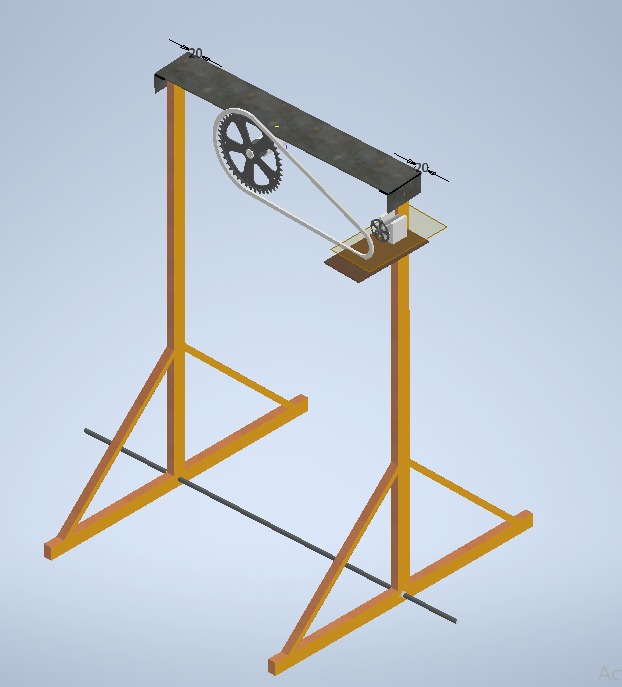
\includegraphics[width=1\linewidth]{A/figs/elements/A_9.jpeg}  


\end{center}
  

\chapter{DIMENSIONAMIENTO DE LARGUERO PRINCIPAL (RIEL)}

\section{Selección de material y/o perfil.} % section headings are printed smaller than chapter names
\makebox[\textwidth]{AISI 1045} \par
Este es un perfil sólido que se encuentra en cualquier distribuidora de metales, el cual se puede comprar por perfil y son bastante largos. Este perfil lo teníamos a nuestro alcance gracias a que un integrante del equipo lo donó para el trabajo, al observar sus características, observamos que cumple con el diseño y gracias a que es un material dúctil, no tanto como el aluminio, se puede observar la deformación .
\\\

\section{Esfuerzo y deformación máxima, (DMF y DEC).}

\begin{table}[htb]
\centering

\begin{tabular}{| p{2.8cm}| p{2.8cm} |}
\hline
\multicolumn{2}{|c|}{AISI 1045} \\
\hline
E &  $\sigma$y \\
\hline \hline
600 MPa & 190-205 GPa  \\ \hline
\end{tabular}
\caption{Propiedades mecánicas}
\label{}
\end{table}

\begin{center}
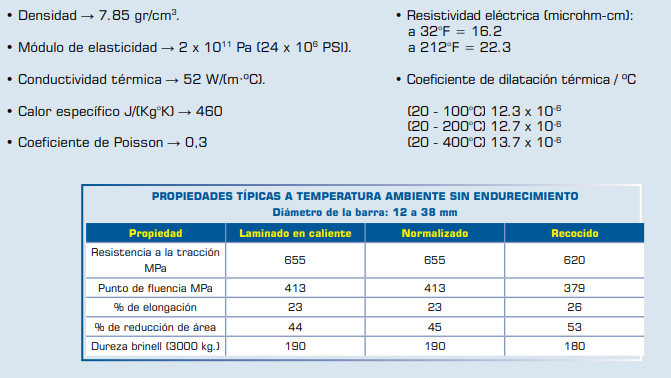
\includegraphics[width=.6\linewidth]{B/figs/B_1.png} 
\end{center}


\subsection{Cargas de diseño}


\begin{equation*}
\textrm{ Polipasto } = 0 .8 \textrm{ Kg}
\end{equation*}
\begin{equation*}
\textrm{ Transmisión} = 0.4 \textrm{ Kg}
\end{equation*}
\begin{equation*}
\textrm{ Elementos para carga } = 5.3 \textrm{ Kg}
\end{equation*}

\subsection{Cálculos de la viga} 

\begin{center}
\includegraphics[width=1\linewidth]{B/figs/C_1.png} 
\end{center}



\begin{align*}
\sigma y & = \frac{M C}{I} \\
        & = \frac{18.11 * 1.58X10^{-3}}{\frac{(0.03175 *  3.17X10^{-3})^{3}}{12}} \\
        & = 339.49 \textrm{ MPa}\\
\end{align*}


\textrm{ con este cálculo se eligió el material que soportará un esfuerzo con un factor}\\ 
\textrm{ de seguridad de}
  
  \begin{align*}
   F.S. & = \frac{600x10^{9}}{339.49} = 1.76 \\
\end{align*}


\begin{center}
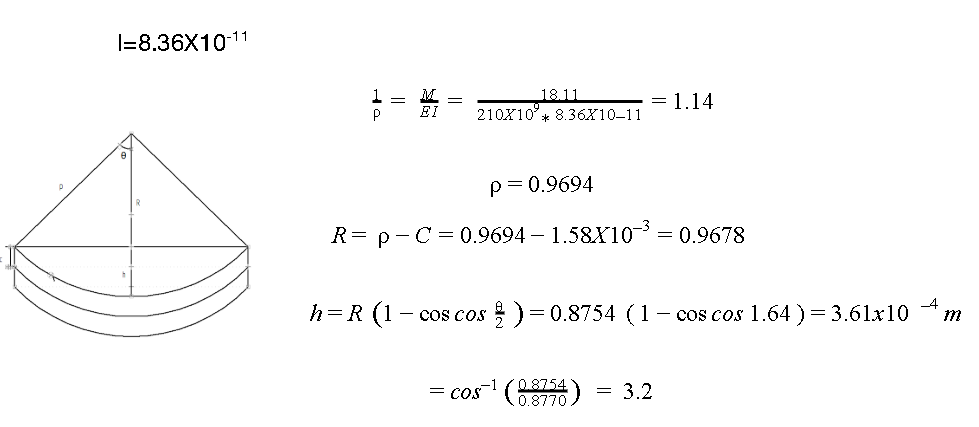
\includegraphics[width=1\linewidth]{B/figs/C_21.png} 
\end{center}

  




\chapter{DIMENSIONAMIENTO DEL CABLE DE CARGA}
\section{Selección de material.} % section headings are printed smaller than chapter names

\makebox[\textwidth]{Hilo – Latón Cu63 Zn37} \par

Se escogió este material ya que es un material bastante sencillo de caracterizar y por supuesto se observa claramente la deformación. Buscamos muchos tipos de hilos, como es de algodón, acero inoxidable etc. , pero el que más se encajaba en cuanto a nuestras características fue este material 
Para la caracterización del material de manera experimental se utilizó el peso que tenemos de base y se fue agregando litro por litro hasta llegar a los 5.300 kg. 

\begin{center}
\includegraphics[width=.3\linewidth]{C/figs/A_1.jpg}
\quad\includegraphics[width=.3\linewidth]{C/figs/A_2.jpg}
\\[\baselineskip]% adds vertical line spacing
\includegraphics[width=.3\linewidth]{C/figs/A_3.jpg}
\quad\includegraphics[width=.3\linewidth]{C/figs/A_4.jpg}
\end{center}

\textrm{Se tomó de base para la caracterización 10 cm exactos, ya agregandole los 5.3 kg se obtuvo un desplazamiento de 1 mm en el cable.}


\section{Esfuerzo y deformación máxima.}

\begin{table}[htb]
\centering
\begin{tabular}{| p{2.8cm}| p{2.8cm} |}
\hline
\multicolumn{2}{|c|}{Latón Cu63 Zn37} \\
\hline
E &  $\sigma$y \\
\hline \hline
100-115 GPa & 300-700 MPa  \\ \hline
\end{tabular}
\caption{Propiedades mecánicas}
\label{}
\end{table}

\begin{center}
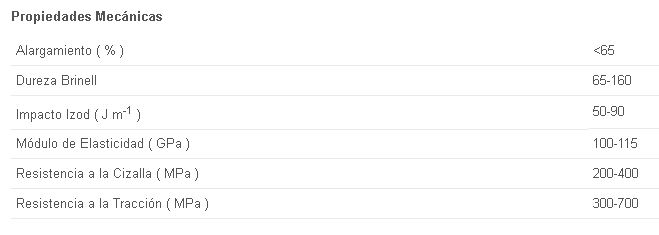
\includegraphics[width=1\linewidth]{C/figs/B_1.jpg} 
\end{center}


\section{Deformación total considerando flexión de \\viga y deformación axial del cable con carga de diseño.}
\begin{center}
\includegraphics[width=.8\linewidth]{C/figs/B_2.jpg} 
\end{center}

  

\chapter{DIMENSIONAMIENTO DEL EJE Y TRANSMISIÓN PARA EL ACCIONAMIENTO DISTANTE DEL POLIPASTO E IZAJE DE LA CARGA A LA MITAD DEL TIRANTE O TRAVESAÑO DE APOYO. }
\begin{center}
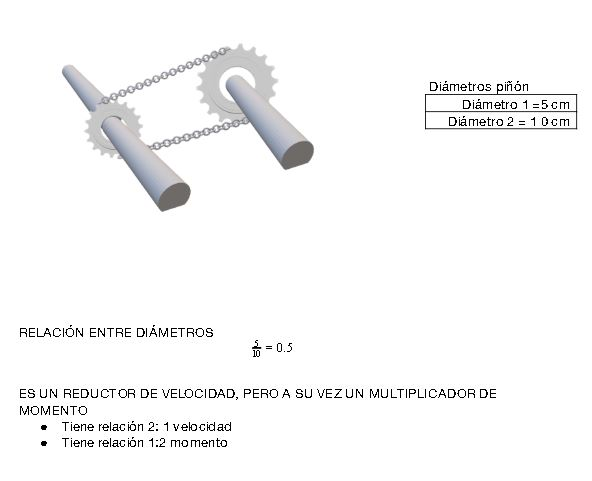
\includegraphics[width=0.9\linewidth]{D/figs/DI_1.jpg} 
\end{center}

\begin{center}
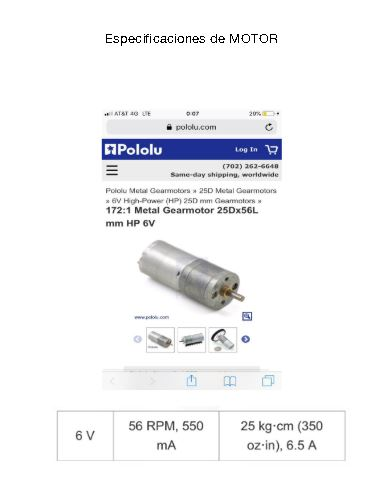
\includegraphics[width=0.7\linewidth]{D/figs/DI_2.jpg} 
\end{center}

\begin{center}
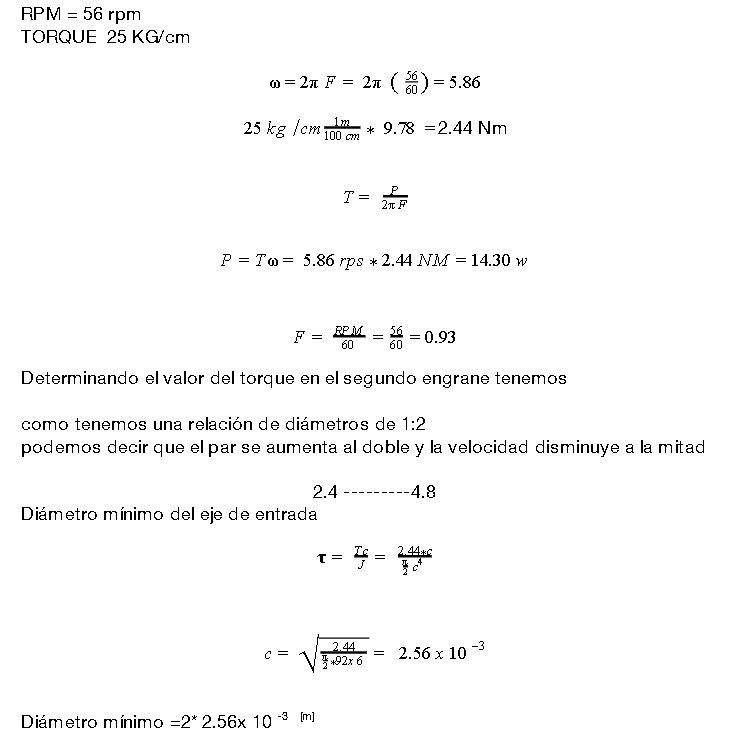
\includegraphics[width=0.9\linewidth]{D/figs/DI_3.jpg} 
\end{center}

\section{Selección del material}

\makebox[\textwidth]{Aluminio} \par
Escogimos aluminio para el eje debido a que tiene las propiedades mecánicas que cumplen con nuestros requisitos. 
\\
\begin{table}[htb]
\centering

\begin{tabular}{| p{2.8cm}| p{2.8cm} | p{2.8cm} |}
\hline
\multicolumn{3}{|c|}{Aluminio} \\
\hline
$\tau$ & E &  G  \\
\hline \hline \hline
92 MPa & 70.6 GPa  & 26.3 GPa \\ \hline
\end{tabular}
\caption{Propiedades mecánicas}
\label{}
\end{table}

\textrm{Se utilizó el $\tau$y= 92 MPa debido a que el valor de esfuerzo de $\sigma$y= 125 MPa}

\textrm{Lo anterior se basa en el siguiente criterio: } \href{http://minisconlatex.blogspot.com/2012/03/guiones-y-comillas.html}{ ``La resistencia a cizallamiento es un valor importante a tener en cuenta para calcular la fuerza necesaria para el corte, así como para determinadas construcciones. No existen valores normalizados a este respecto, pero generalmente es un valor que está entre el 55 y 80 porciento de la resistencia a la tracción.''}

\bigskip
\bigskip
\bigskip
\bigskip
\textrm{Módulo de elasticidad longitudinal o Módulo de Young}

\begin{center}
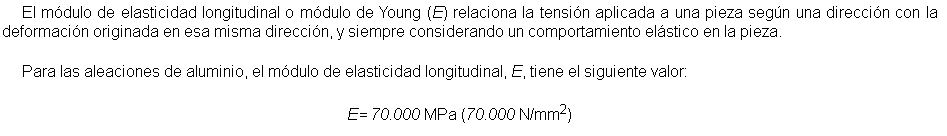
\includegraphics[width=0.9\linewidth]{D/figs/D_3.jpg} 
\end{center}


\textrm{de acuerdo con el proveedor del material tenemos}
\begin{center}
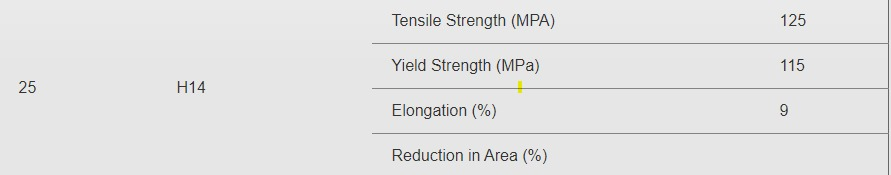
\includegraphics[width=0.9\linewidth]{D/figs/D_4.jpeg} 
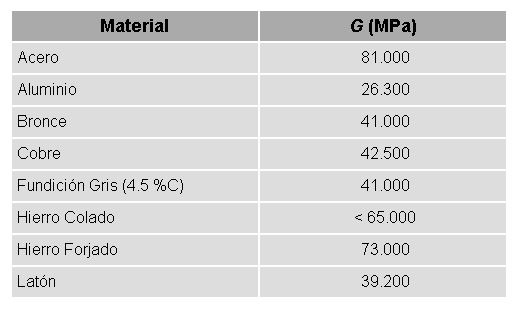
\includegraphics[width=0.9\linewidth]{D/figs/D_5.jpg} 
\end{center}

\section{Esfuerzo y Deformación máxima, (DMF y DEC).}

\begin{table}[htb]
\centering
\begin{tabular}{| p{2.2cm}| p{2.2cm} |}
\hline
\multicolumn{2}{|c|}{Aluminio} \\
\hline
E & G \\
\hline \hline
70 GPa & 26.3 GPa  \\ \hline
\end{tabular}
\caption{Propiedades mecánicas}
\label{}
\end{table}


\section{Determinación de diámetro.}

\begin{center}
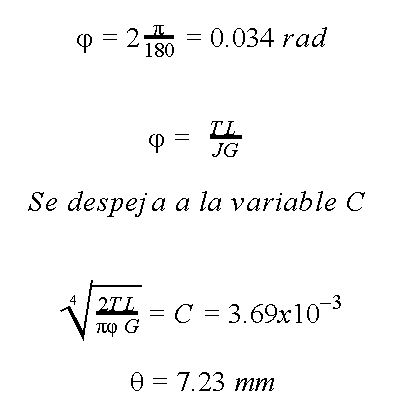
\includegraphics[width=0.6\linewidth]{D/figs/DB_1.jpg} 
\end{center}

\begin{equation*}
\textrm{ Diámetro } = 8 \textrm{ mm }
\end{equation*}
\begin{equation*}
\textrm{ Longitud } = 10 \textrm{ cm}
\end{equation*}
\begin{equation*}
\textrm{ Radio } = 4 \textrm{ mm }
\end{equation*}

\begin{equation} 
\begin{split}
\tau & = \frac{T C}{J} \\
\end{split}
\end{equation}


\begin{center}
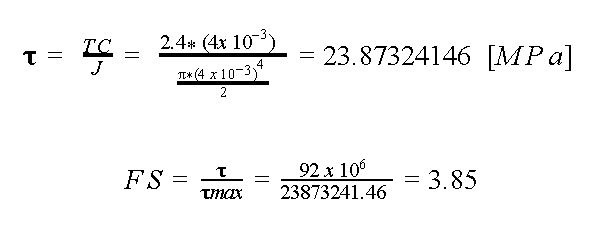
\includegraphics[width=0.6\linewidth]{D/figs/DB_2.jpg} 
\end{center}


\section{Deformaciones en el eje.}

\begin{equation} 
\begin{split}
J & = \frac{\pi C^2}{2} \\
  & = \frac{\pi (8x10^{-3})^2}{2} \\
  & = 1.0052x10^{-4} [m^{4}]\\
\gamma & = \frac{2.4516625*8x10^{-3}}{1.0052x10^{-4}*26.3x10^{9}} \\
       & = 7.4181x10^{-9} [rad]\\
       & = 4.25x10^{-9} [grados]
\end{split}
\end{equation}  


\chapter{MEDICIÓN Y DEMOSTRACIÓN DE RESULTADOS EXPERIMENTALES.}

\section{A través de medios electrónicos o mecánicos, de al menos los puntos b), c) y d).
}

\subsection{Sensor de proximidad}
\href{https://youtu.be/l9V6qCGNVYA}{En este video } \textrm{: se puede apreciar un demo de cómo mediremos la deformación de la viga.}
\bigskip
\bigskip
\begin{center}
\includegraphics[width=.8\linewidth]{E/figs/A_1.jpg} 
\end{center}
\bigskip
\bigskip
\bigskip
\bigskip
\bigskip

\subsection{Bot telegram}
\textrm{ De ser posible también tendremos un Bot que nos dará las métricas de todos los puntos solicitados}

\begin{center}
\includegraphics[width=.6\linewidth]{E/figs/A_2.jpg} 
\end{center}  


\chapter{RESULTADOS Y CONCLUSIONES}

\section{Análisis y ponderación de resultados \\de con \%E <10\%.}


En este \href{https://bit.ly/37uKJzo}{link está nuestro proyecto interactivo} : se pueden modificar valores y todo se recalcula nuevamente.
\\La versión final de nuestro trabajo estará disponible es este \href{https://erickbarcenas.github.io/Polipasto/}{sitio web}.

\subsection{Pre-conclusiones}
Este proyecto nos ayudó a trabajar los conceptos que estudiamos a lo largo del curso tales como esfuerzo de diseño, cargas, deformaciones etc., de esta forma nos quedó clara la aplicación de cada uno. Por otro lado, nos sirvió también para ver la magnitud que conlleva al trabajar en un problema de diseño desde escoger materiales hasta la manufactura del proyecto, independientemente de que aplicación se le vaya a dar.
Nos deja preparados para afrontar problemas de este tipo en el futuro a lo largo de nuestra carrera, al menos para tener una idea de cómo plantearlo y trabajar en él.
También observamos que al tratarse de un polipasto que debe soportar cierta carga se requiere tener cuidado con los cálculos ya que ligeras diferencias se ven reflejadas en la maqueta, por lo que son de gran importancia ya que la industria puede significar tiempo y dinero.
A lo largo del proceso de realización de este polipasto no hemos topado con demasiados problemas que se han resuelto poco a poco, como son, la elección del material, y sin duda la elección de un motor que se pueda caracterizar. 

Los polipastos son una herramienta que facilita la convención de elementos de gran peso sin la necesidad de utilizar un gran despliegue de fuerza; En nuestro caso está hecho con una transmisión, hecha de piñones de bicicleta. Al realizar el polipasto en físico nos hemos enfrentado a problemas como la soldadura y el armado de la estructura ya que no se cuentan con los conocimientos necesarios para no echar a perder el material, sin embargo, siempre podemos pedir ayuda y resolver los problemas.

Al investigar sobre su funcionamiento nos hemos dado cuenta de que los polipastos han sido una valiosa invención que ha contribuido enormemente en la evolución industrial, sin comentar que las investigaciones actuales están llevando a la creación de polipastos tan avanzados que la carga de un edificio entero dejara de ser un sueño dentro de algunos años, y pasará a ser una realidad gracias a los nuevos materiales que se están implementado en la investigación de los polipastos en este momento.

  

\chapter*{FUNETES DE CONSULTA}

\href{https://ingemecanica.com/tutorialsemanal/tutorialn110.html}{Propiedades mecánicas para el eje }

\href{http://www.rmmcia.es/blog/laton-y-cobre/propiedades-del-laton}{Propiedades mecánicas para el hilo }

\href{https://repository.unilibre.edu.co/bitstream/handle/10901/7826/VasquezTorresEdwinLibardo2013Anexos.pdf?sequence=2}{Propiedades mecánicas para el perfil }







\end{document}
%Á á, É é, Í í,Ó ó,Ú ú,Ü ü,Ñ ñ, ¿, ¡ ``